
\subsubsection{Simulated ECal Occupancies and Acceptance}
Description of occupancy and acceptance for the ECal.

\subsubsection{Simulated Tracker Occupancies and Acceptance}
Description of the expected occupancies and acceptance in the SVT from simulation.

\subsection{Simulation of backgrounds and detector occupancies}
\label{sec:backgrounds}

\subsubsection{ECal occupancies}

There are two factors limiting the allowable ECal occupancy. First, the ECal readout algorithm uses a window of fixed size to integrate hit energy. This window was set to 140 ns ($35 \times 4$ ns) for the test run, and so the number of hits above readout threshold in a 140-ns time window should be well below 1. Figure \ref{fig:ecal_rate} shows that the maximum rate in any crystal is 500 kHz, which translates to 0.07 hits in 140 ns.

Second, because the FADC only reads out on a rising threshold crossing, each hit above threshold causes dead time for that crystal until the preamp output falls back below threshold. Figure \ref{fig:ecal_deadtime} shows the fraction of time each crystal spends above threshold. The maximum dead time is 0.03, meaning that even the hottest crystal is sensitive to new hits 97\% of the time.

\begin{figure}[ht]
	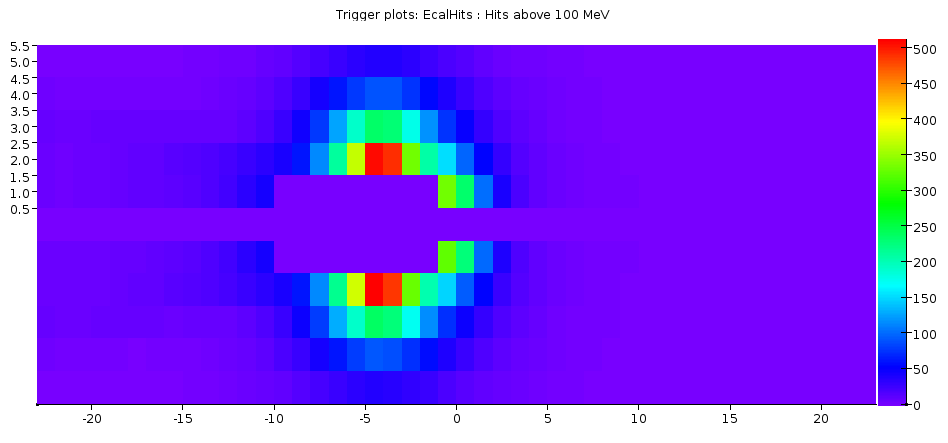
\includegraphics[width=\textwidth]{performance/ecal_rate_100mev_22}

	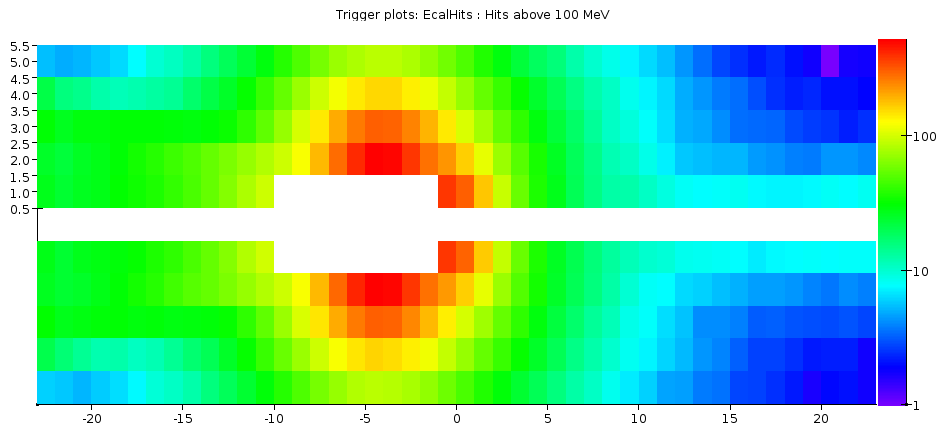
\includegraphics[width=\textwidth]{performance/ecal_rate_100mev_22_log}
	\caption{\small{Rate of hits over 100 MeV (units of kHz) per crystal. Top plot uses linear scale for the Z-axis; bottom plot is log scale.}}
	\label{fig:ecal_rate}
\end{figure}

\begin{figure}[ht]
	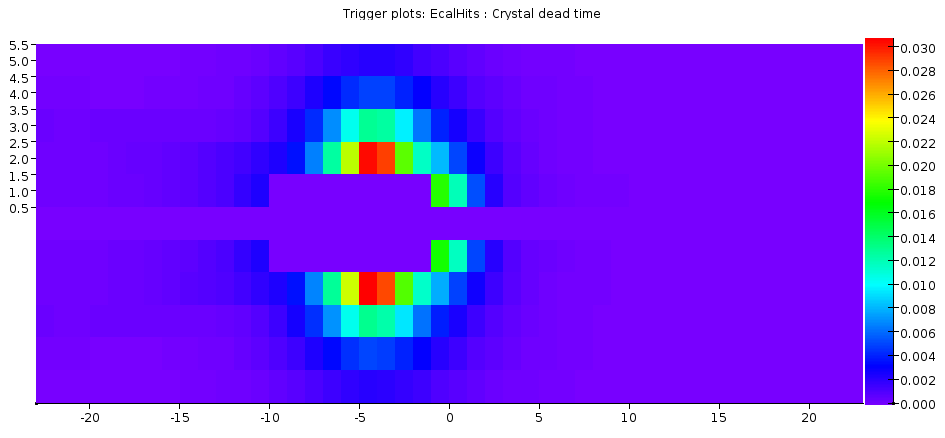
\includegraphics[width=\textwidth]{performance/ecal_deadtime_22}
	\caption{\small{ECal readout deadtime fraction for 2.2 GeV running, with a threshold of 75 MeV for each crystal.}}
	\label{fig:ecal_deadtime}
\end{figure}

\subsection{Trigger rates: ECal and muon detector}
\subsubsection{ECal trigger performance}

The proposed ECal trigger was simulated to test trigger cuts, verify that the trigger has acceptable efficiency for A' events, and verify that the trigger rate is compatible with the HPS DAQ in all running conditions.

Trigger simulation is done in three stages. 
First, various packages are used to simulate beam interactions in the target---details are given in Section \ref{sec:backgrounds}.
The beam background files (equivalent to 100 ms of beam at each energy) are merged into a common StdHep format. 
A' tridents are also simulated using MadGraph. 
Next, the Geant4-based simulations system SLIC \cite{slic} is used to simulate interactions and energy deposition in the magnetic field, tracker, vacuum chamber and ECal. 
Finally, readout and trigger simulation is done using LCSim.
This is a faithful simulation of the detector, DAQ and trigger and has been tested against the actual performance of the test run detector and DAQ. See Section \ref{sec:triggerdaq} for details of the readout, clustering and trigger algorithms.

The trigger parameters described in Section \ref{sec:triggerdaq} are chosen by running the simulation and plotting the relevant variables for beam background and A' events. 
This is done for each beam energy and a set of A' masses for each beam energy. Examples of these comparisons are shown in Figures \ref{fig:coplanarity}, \ref{fig:energy-distance} and \ref{fig:ediff}.

\begin{figure}[ht]
	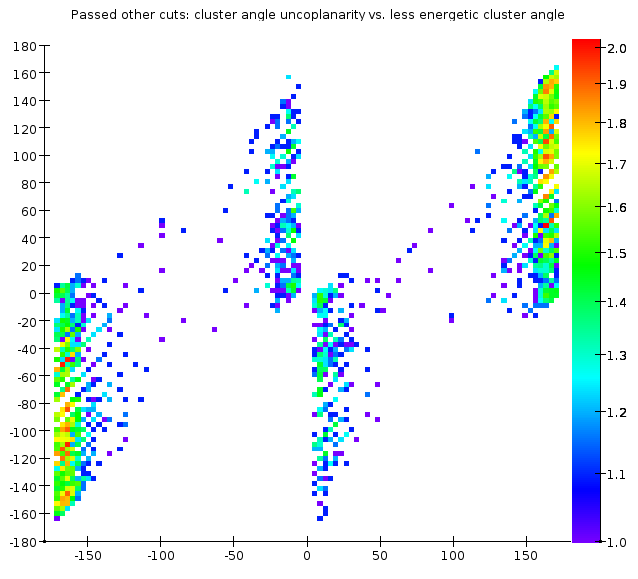
\includegraphics[width=0.4\textwidth]{performance/coplanarity_22}
	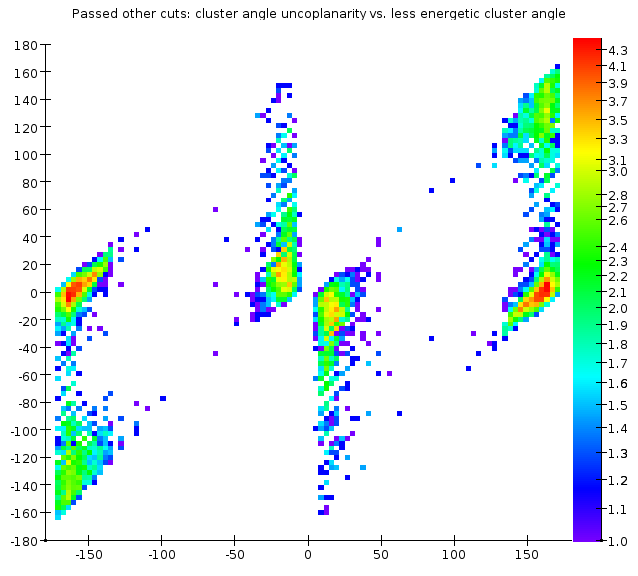
\includegraphics[width=0.4\textwidth]{performance/coplanarity_22_075mev}
	\caption{\small{Deviation of cluster pairs from coplanarity (units of degrees), for 2.2 GeV background and 75 MeV A' tridents.}}
	\label{fig:coplanarity}
\end{figure}

\begin{figure}[ht]
	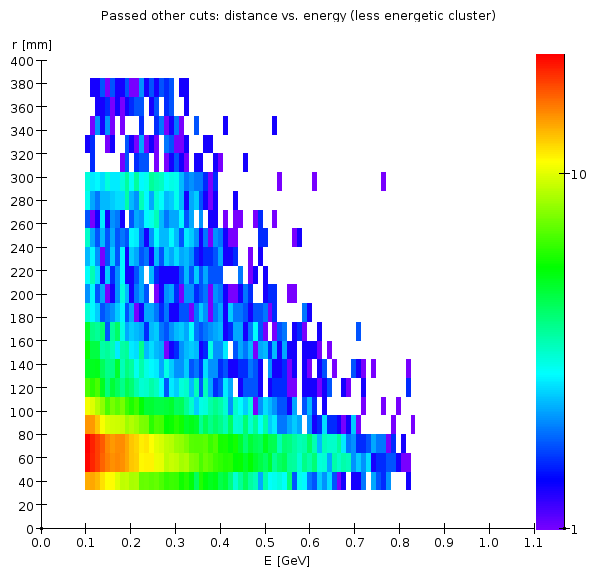
\includegraphics[width=0.4\textwidth]{performance/energy-distance_22}
	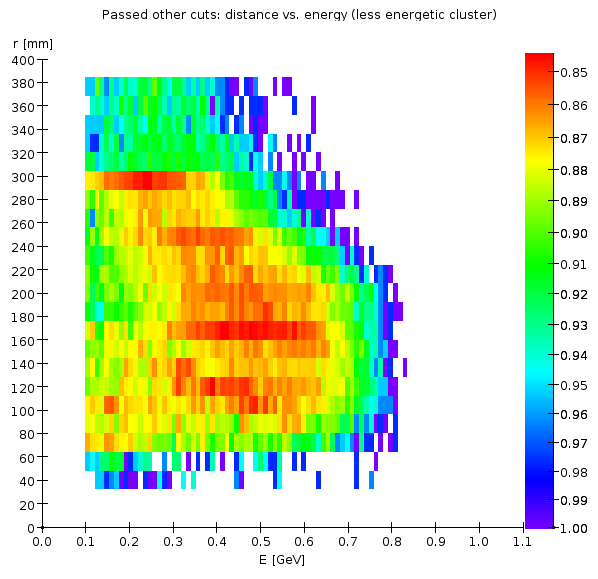
\includegraphics[width=0.4\textwidth]{performance/energy-distance_22_075mev}
	\caption{\small{Energy and distance from beam axis of the lower-energy cluster, for 2.2 GeV background and 75 MeV A' tridents.}}
	\label{fig:energy-distance}
\end{figure}

\begin{figure}[ht]
	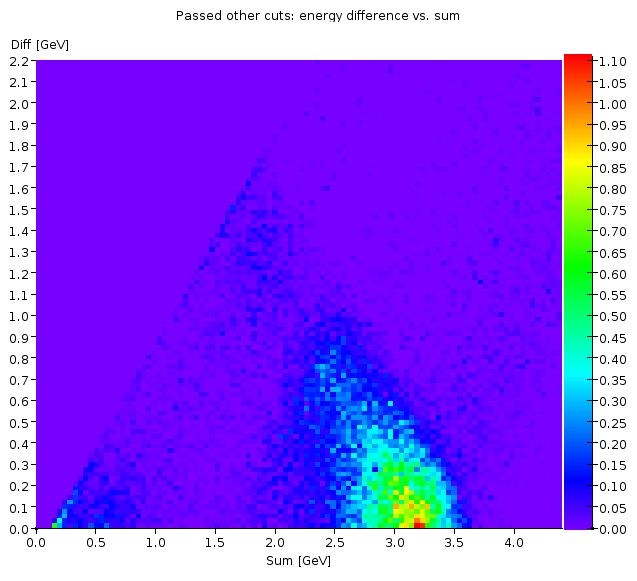
\includegraphics[width=0.4\textwidth]{performance/ediff_22}
	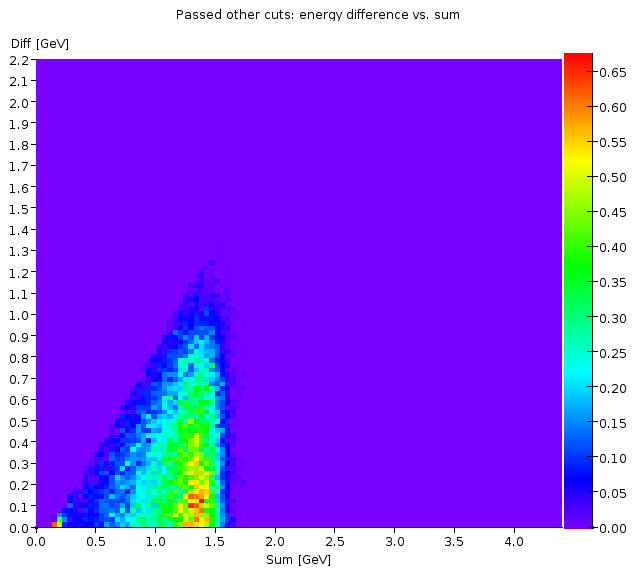
\includegraphics[width=0.4\textwidth]{performance/ediff_22_075mev}
	\caption{\small{Energy sum and difference of cluster pairs, for 2.2 GeV background and 75 MeV A' tridents.}}
	\label{fig:ediff}
\end{figure}

The following trigger parameters were determined to be independent of beam energy:
\begin{itemize}
	\item Minimum cluster energy ($E_{min}$): 0.1 GeV
	\item Energy-distance distance ($r_{edist}$): 200 mm
	\item Energy-distance energy ($E_{edist}$): $0.5\times E_{beam}$
\end{itemize}

The remaining trigger parameters given in Section \ref{sec:triggerdaq} do not have a significant effect on specificity of the trigger.

\begin{table}
	\begin{tabular}{|l|r|r|r|}
		\hline
		Beam energy [GeV] & $E_{max}$ [GeV] & $Esum_{max}$ [GeV] & $\Delta\phi_{max}$ [$^\circ$] \\
		\hline
		1.1	&	0.7	&	0.8	&	90\\
		2.2	&	1.6	&	1.7	&	45\\
		6.6	&	5.0	&	5.5	&	60\\
		\hline
	\end{tabular}
	\caption{ {\small Trigger parameters optimized for different beam energies.}
	\label{tab:trigcuts}}
\end{table}

Trigger efficiency for A' events is defined as the fraction of A' tridents (generated without fiducial cuts) that produce a trigger.

Trigger rates are shown in Table \ref{tab:trigrates}. These rates are safely under the maximum readout rate of 43 kHz set by the SVT. 
The addition of pions to the 6.6 GeV background sample does not have a significant effect on the trigger rate.

\begin{table}
	\begin{tabular}{|l|r|}
		\hline
		Sample &  Rate (kHz)\\
		\hline
		1.1 GeV	EGS5 				& 15.7 $\pm$ 0.4	\\
		1.1 GeV EGS5+tridents			& 17.6 $\pm$ 0.6	\\
		2.2 GeV	EGS5 				& 11.2 $\pm$ 0.3	\\
		2.2 GeV EGS5+tridents			& 15.8 $\pm$ 0.4	\\
		6.6 GeV	EGS5 				& 10.2 $\pm$ 0.3	\\
		6.6 GeV EGS5+tridents			& 12.6 $\pm$ 0.4	\\
		%6.6 GeV EGS5+tridents+pions (FLUKA)	& 7.3 $\pm$ 0.3	\\
		%6.6 GeV EGS5+tridents+pions (G4)	& 7.0 $\pm$ 0.3	\\
		\hline
	\end{tabular}
	\caption{ {\small Trigger rates using various background samples. }
	\label{tab:trigrates}}
\end{table}

Trigger efficiency for A' events is defined as the fraction of A' tridents (generated without fiducial cuts) that produce a trigger.

For the performance of the experiment, we are interested in the combined efficiency of the trigger and tracker: the fraction of A' tridents that produce a trigger and leave enough hits in the tracker for a pair of tracks to be reconstructed.
We simulate charge deposition and readout of the tracker (turning off the generation of noise hits), and check each sensor for hits. 
If the DAQ reads out hits in four stereo pairs in each half of the tracker, the event is in the combined acceptance.

Both efficiency values (trigger only, and combined) are shown in Figure \ref{fig:trigeff}. 
Both trigger and tracker acceptances are dominated by the geometric acceptances of the ECal and tracker.

\begin{figure}[ht]
	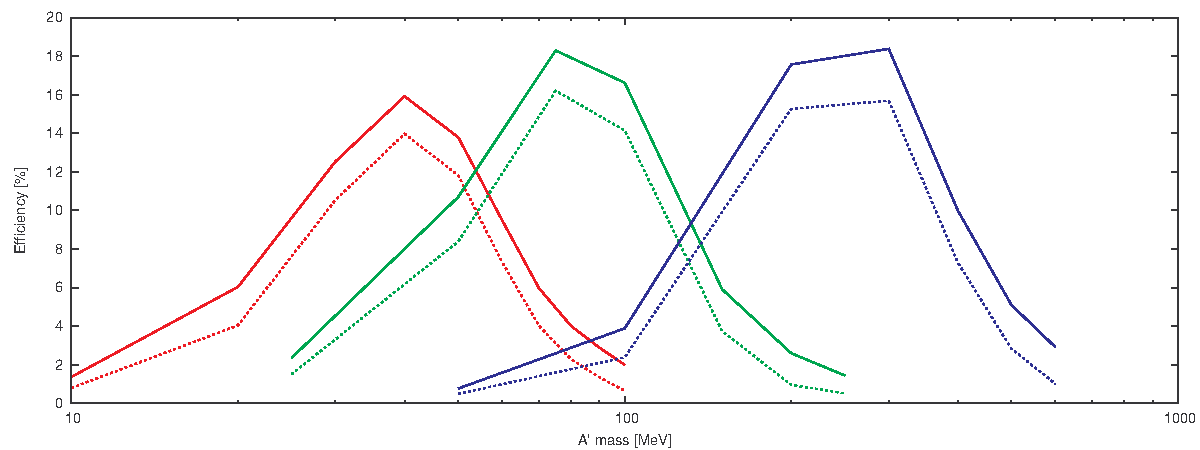
\includegraphics[width=\textwidth]{performance/ap_eff}
	\caption{\small{Trigger efficiency (solid lines) and combined efficiency (dashed lines) as a function of A' mass, at beam energies of 1.1, 2.2 and 6.6 GeV (red, green and blue respectively).}}
	\label{fig:trigeff}
\end{figure}

\subsubsection{Muon trigger performance}

\subsection{Track reconstruction}

\subsection{Cluster reconstruction}

\subsection{Muon identification}

